%! TeX root = ../phd-thesis.tex
%! Author = davidedomini

%----------------------------------------------------------------------------------------
\chapter{Introduction}
\label{chap:introduction}
\minitoc
%----------------------------------------------------------------------------------------

\section{Context}

The last decade has seen a rapid growth in the number 
 of networked devices embedded in physical environments,
 bringing the long-standing visions of 
 ubiquitous~\cite{DBLP:journals/sigmobile/Weiser03}, 
 pervasive~\cite{DBLP:journals/computer/SahaM03}, 
 everywhere~\cite{DBLP:journals/newriders/adam}
 and collective~\cite{DBLP:journals/computer/Abowd}
 computing increasingly close to reality. 
% 
These devices continuously generate data,
 communicate with one another, and increasingly make autonomous decisions.
%
Rather than operating in isolation, 
 they form distributed systems that support applications such as 
 smart cities, pervasive sensing, autonomous mobility, robotic collectives, 
 and the edge--cloud continuum.

The behaviour of these systems cannot be understood solely 
 in terms of their individual components. 
% 
Each device acts on the basis of partial information, 
 derived from its local state and from interactions with a limited 
 and possibly changing set of neighbours. 
%
Nevertheless, 
 these locally situated actions influence one another 
 and jointly give rise to the behaviour observed at the system level. 
% 
This interplay between local autonomy 
 and system-level emergence is characteristic of \glspl{CAS}: 
 systems composed of multiple autonomous or semi-autonomous entities that interact locally, 
 adapt during operation, and pursue individual or collective objectives.

Autonomy in these systems can be engineered through different, 
 and potentially complementary, approaches.
%
Explicit programming approaches include agent-level architectures, 
 such as belief--desire--intention models, 
 and macroprogramming abstractions that allow collective behaviour 
 to be specified from a global perspective.
%
Learning-based approaches instead derive models or decision policies 
 from data and experience.
%
For example, 
 \gls{MARL} enables agents 
 to learn through interactions with one another and their environment, 
 while \gls{FL} allows distributed devices to construct shared models 
 without centralizing their raw data.

Regardless of the approach, 
 engineering these systems is complicated by both scale and dynamism.
%
A collective may comprise hundreds or thousands of devices, 
 motivating the term \emph{many-agent} for settings whose scale is substantially larger 
 than that usually associated with small multi-agent systems (i.e., two to ten agents).
%
Moreover, 
 the collective is rarely static: 
 devices may move, fail, join, or leave during operation, 
 causing both the communication topology and the information available 
 within the system to evolve.

When autonomy relies on learning, 
 an additional challenge arises from the way data are generated and collected.
%
Because each device observes only a particular portion of the physical environment, 
 local datasets rarely satisfy the common \gls{IID} assumption.
%
This heterogeneity is often spatially structured: 
 devices exposed to the same local phenomenon may observe related distributions, 
 whereas devices operating in different regions or contexts may collect 
 substantially different data.
%
Furthermore, 
 mobility and changes in the underlying phenomena 
 may cause these distributions and their spatial organization to evolve over time. 

\section{Motivating Scenarios}

\paragraph{Cooperative autonomous mobility.}
Consider a metropolitan area populated by 
 autonomous vehicles, roadside units, and edge servers. 
% 
Each vehicle observes local traffic conditions 
 and uses this information to forecast congestion and select an appropriate route. 
% 
However, 
 no vehicle has a complete view of the road network: 
 observations collected by other vehicles can improve its predictions, 
 while the routes selected across the fleet jointly shape the traffic conditions 
 that will subsequently be observed. 
% 
This creates a continuous feedback loop between local observations, 
 individual decisions, and system-level behaviour.

Useful information is not uniformly distributed across the fleet. 
%
Traffic patterns vary across districts, roads, directions, and times of day, 
 and may change abruptly because of accidents, weather, or public events. 
% 
Consequently,
 information obtained in one context may be of limited value in another, 
 and the vehicles from which an agent can benefit may change as it moves through the city. 
% 
Cooperation must therefore adapt to both the spatial distribution 
 of traffic conditions and their evolution over time.

Collecting all observations at a central location would raise 
 privacy, communication, latency, and scalability concerns. 
% 
Computation is also distributed: 
 latency-critical operations may run on board, 
 more demanding tasks may be delegated to nearby edge infrastructure,
 and delay-tolerant processing may use cloud resources. 
% 
These choices depend on local connectivity, workload, and hardware capabilities, 
 but are also coupled through shared communication and computational resources. 
% 
Effective operation therefore requires vehicles to coordinate learning 
 and resource usage without relying on complete global knowledge.

\paragraph{Disaster-response collectives.}
A complementary scenario arises after a natural disaster, 
 when aerial drones, ground robots, environmental sensors, 
 and portable edge stations cooperate to map damaged areas, detect hazards, 
 and locate people. 
% 
Each device observes only a limited portion of the environment 
 and can communicate only with currently reachable neighbours. 
% 
Building an operational picture therefore requires
 combining observations collected at different locations and times.

In this setting, 
 neither the population nor the supporting infrastructure can be assumed to remain stable. 
% 
Devices may move, become disconnected, exhaust their batteries, or fail, 
 while hazards and accessibility conditions evolve throughout the emergency. 
% 
At the same time, 
 transmitting high-resolution sensor data may consume scarce energy and bandwidth, 
 whereas individual devices may lack the resources required to process it locally. 
% 
The collective must thus decide how to distribute sensing, learning, 
 and computation while continuing to operate under changing and incomplete information.

Together, 
 these scenarios illustrate the central engineering challenge addressed in this thesis.
% 
Learning is not performed by isolated devices within a fixed environment, 
 but is embedded in a dynamic collective whose members, interactions, knowledge, 
 and resources evolve during operation. 
% 
Achieving desirable system-level behaviour consequently requires coordinating 
 how agents learn from one another, how their decisions account for neighbouring agents,
 and how computation is distributed across the available infrastructure.
 
\section{Research Gap}

Existing approaches to engineering distributed and adaptive systems make
different choices about how the system and its components are represented. Some
adopt the individual device as their main abstraction, whereas others describe
the collective as a whole. Components may be modelled as passive computational
objects or as autonomous agents. Their coordination may be centralized,
decentralized, or hybrid, and adaptive behaviour may be expressed through
rules, optimization objectives, learned models, or decision policies. These
choices determine what information is available to each component, where
decisions are made, and how system-level behaviour can be controlled.

Macroprogramming and machine learning address complementary parts of this
design space. Macroprogramming provides abstractions for constructing robust
collective behaviour from local interactions; machine learning enables models
and policies to adapt from data or experience. Their integration, however, is
still fragmented. Distributed learning algorithms are commonly studied under a
predefined coordination architecture, communication topology, participation
model, and deployment environment. Conversely, programming abstractions for
collectives do not by themselves determine how models should be trained, how
collaborators should be selected, or how learning tasks should be placed on
heterogeneous resources. Embedding learning in a CAS exposes four coupled
engineering dimensions, summarized in~\Cref{fig:overview}.

\begin{figure}
    \centering
    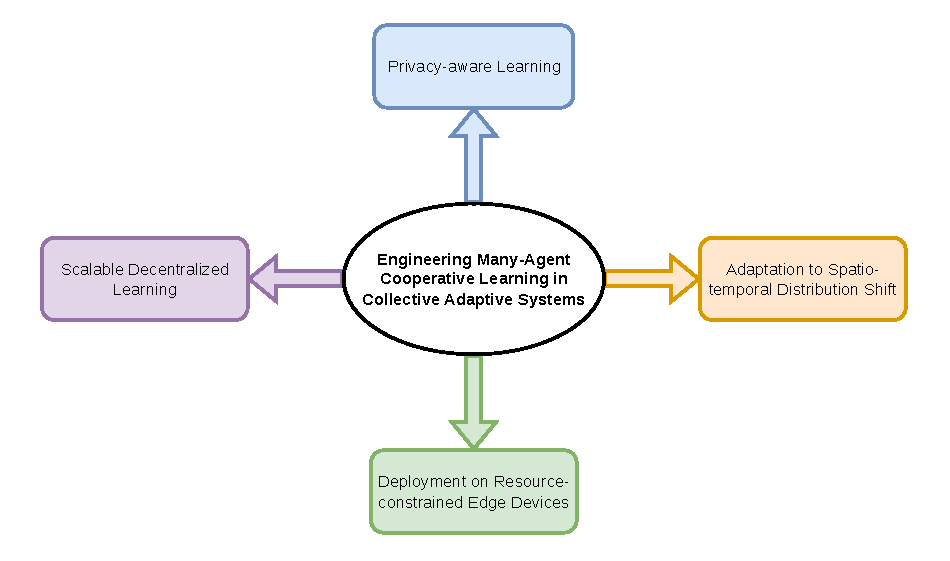
\includegraphics[width=0.9\textwidth]{figures/axes.drawio.pdf}
    \caption{Engineering dimensions that arise when cooperative learning is embedded in a Collective Adaptive System.}
    \label{fig:overview}
\end{figure}

\emph{Data privacy constraints} concern how agents can benefit from distributed
observations without requiring raw, potentially sensitive data to be collected
at a central location. In the mobility scenario, route histories and
destinations should remain on the vehicles; in disaster response, raw imagery
may reveal people or private spaces. Retaining data locally motivates FL, but
data location alone is not a complete privacy design: model updates and derived
information may also disclose properties of local observations, and the chosen
aggregation structure determines which participants receive them. The
engineering problem therefore includes what information is exchanged, within
which collaboration boundary, and under which coordination and trust model.

\emph{Spatio-temporal distribution shift} concerns the fact that the data
observed by agents are structured by both location and time. Traffic samples
from a highway and a city centre are not interchangeable, while a moving
vehicle encounters a sequence of local distributions. Likewise, robots deployed
in different disaster zones experience different sensing conditions, and those
conditions evolve during the mission. Spatial proximity can be useful evidence
of statistical similarity, but it is not sufficient on its own. Learning must
support localized models, revise collaboration boundaries when context changes,
and retain useful knowledge across transitions. This is a systems concern as
well as a statistical one, because adapting a model may require adapting the
topology and membership of the learning process that produces it.

\emph{Scalable decentralization} concerns how learning and coordination can rely
on local interactions while remaining effective as the collective grows and its
communication graph changes. A central server coordinating a metropolitan fleet
would be a communication bottleneck and a single point of failure; after a
disaster, such a server may not be reachable at all. Yet removing it transfers
responsibilities such as collaborator discovery, aggregation, role election,
and recovery to the devices. These mechanisms must work without global
knowledge and without assuming a fixed number or ordering of agents.
Macroprogramming is relevant precisely at this boundary: system-level patterns
such as regions, information gradients, and temporary leaders can be specified
once and realized through repeated local interactions. The open question is how
such patterns should be composed with learning algorithms and how learned
policies themselves can generalize across collective sizes.

\emph{Resource-constrained edge devices} concern the computational, memory,
energy, and communication limitations that restrict training and inference at
the network edge. An onboard computer or battery-powered robot may be unable to
train a dense model frequently or transmit it over a low-bandwidth link. Model
sparsification, communication-efficient learning, and task offloading can reduce
these costs, but their effect depends on the collective context. A smaller model
may change which devices appear statistically similar; offloading may save local
energy while increasing shared network congestion; and selecting a remote
resource may violate an application's latency bound. Resource feasibility is
therefore not only a property of an individual model or device, but also an
emergent property of concurrent decisions across the system.

The four dimensions cannot be engineered independently. In the mobility
scenario, reducing communication may slow the reorganization of learning
federations; changing federation membership may affect both specialization and
the exposure of model information; and sending training to an edge server may
relieve a vehicle while overloading the infrastructure used by its neighbours.
Similar dependencies arise when failures fragment a disaster-response network.
An optimization performed within one layer can consequently move cost or risk
to another layer rather than remove it.

The research gap is thus not a lack of individual algorithms for federated
learning, multi-agent reinforcement learning, self-organization, or offloading.
It is the lack of a systematic way to engineer them around the defining
properties of CASs, so that the coordination structure, learning architecture,
adaptation mechanism, and deployment strategy are designed as parts of the same
system. Existing work often addresses one dimension in isolation or introduces
an application-specific solution under fixed assumptions about the others. What
remains needed are reusable coordination mechanisms, scalable learning
architectures, and deployment strategies that bridge collective-level intent and
device-level execution. Accordingly, this thesis treats cooperative learning as
an integral part of the CAS rather than as an algorithmic component added after
the surrounding system has been designed.


\section{Contribution}

\begin{figure}
    \centering
    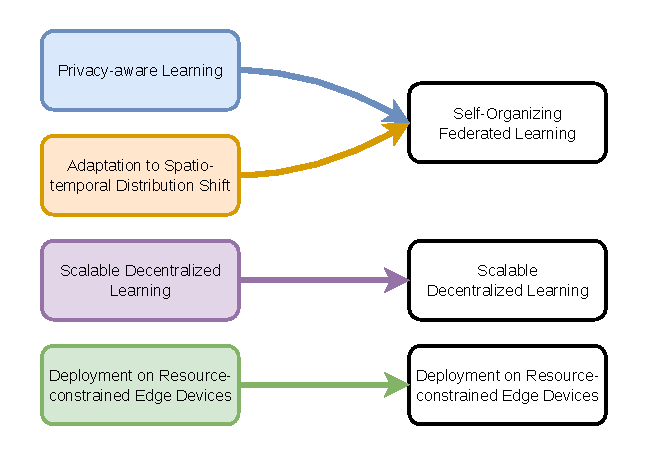
\includegraphics[width=0.9\textwidth]{figures/mapping.drawio.pdf}
    \caption{Relationship between the engineering dimensions and the contribution chapters of this thesis.}
    \label{fig:mapping}
\end{figure}

Starting from the research gap outlined above, this thesis investigates how
cooperative learning can be engineered as an integral part of a CAS. The
objective is not to define a single learning algorithm for every collective
system, but to identify coordination mechanisms, learning architectures, and
deployment strategies that remain viable under distribution, locality, scale,
openness, and resource constraints. Particular attention is given to the role of
macroprogramming in expressing self-organizing structures around a learning
process, and to architectures that avoid encoding a fixed collective size in the
learned solution.

The investigation is guided by the following research questions:

\begin{questions}
\item
How can privacy-aware cooperative learning be organized among many distributed
agents without centralizing raw data or relying on a fixed central coordinator?
\label{itm:rq1}

\item
How can cooperative learning account for spatially heterogeneous data and adapt
to temporal distribution shifts caused by mobility and changing environments?
\label{itm:rq2}

\item
How can decentralized learning remain effective and scalable when agents have
access only to local observations, communicate with a limited neighbourhood,
and operate in collectives whose size may change?
\label{itm:rq3}

\item
How can learning-based decisions be deployed across heterogeneous and
resource-constrained edge--cloud infrastructures while accounting for both
individual device constraints and collective system-level phenomena?
\label{itm:rq4}

\end{questions}

These questions are addressed through three complementary lines of research,
whose relationship with the engineering dimensions is summarized
in~\Cref{fig:mapping}.

The first line concerns \emph{self-organizing federated learning} and
addresses~\ref{itm:rq1} and~\ref{itm:rq2}. Field-based coordination mechanisms
are used to let devices construct and maintain learning federations according to
spatial proximity and model similarity, without a fixed server or prior
knowledge of the number of groups. This line introduces localized learning
methods, evaluates their robustness to changes in topology and participation,
and provides a benchmark for spatially structured data heterogeneity. It also
studies how federations and models can adapt to mobility-induced distribution
shifts while retaining previously acquired knowledge, and how model
sparsification can reduce computation and communication costs without removing
the spatial structure of collaboration.

The second line addresses~\ref{itm:rq3} through \emph{scalable decentralized
reinforcement learning}. It investigates training strategies based on
interactions among neighbouring agents and learning architectures that operate
on variable-sized neighbourhoods. The resulting analysis characterizes the
trade-offs between centralized training, independent learning, and local
cooperation, and examines whether policies trained with a given number of
agents remain effective when deployed in larger collectives.

The third line concerns \emph{adaptive deployment across the edge--cloud
continuum} and addresses~\ref{itm:rq4}. It develops a learning-based approach
through which devices make decentralized application placement and offloading
decisions. The method combines local information, including energy and
computational capacity, with collective conditions such as latency, network
congestion, and infrastructure load, thereby accounting for the externalities
created by concurrent device decisions.

Together, these contributions surround learning with explicit coordination and
deployment mechanisms instead of treating it as an isolated algorithm. They
provide concrete methods and broader design evidence for
integrating learning into many-agent systems with distributed data, local
interactions, dynamic populations, and limited resources.


\section{Thesis Structure}

The remainder of this thesis is organized into two main parts.

\emph{Part~I---Background} introduces the concepts required to frame the
contributions. \Cref{chap:context} presents Collective Adaptive Systems,
self-adaptive systems, and the edge--cloud continuum, establishing the
computational and deployment setting considered throughout the thesis.
\Cref{chap:macroprogramming} introduces macroprogramming and the abstractions
used to express collective behaviour through local interactions.
\Cref{chap:ml} provides the machine-learning foundations required by the
subsequent chapters. \Cref{chap:federated-learning} focuses on federated
learning, with particular attention to decentralized architectures, non-IID data,
and clustered approaches. \Cref{chap:reinforcement-learning} introduces
reinforcement learning and its extension to multi-agent settings, including
decentralized training and scalability.

\emph{Part~II---Contribution} presents the research developed during this
thesis. \Cref{chap:selforg-fl} introduces the proposed approaches to
self-organizing federated learning, from spatial federation formation to
adaptation under mobility and resource constraints. \Cref{chap:scalable-rl}
investigates scalable decentralized reinforcement learning, focusing on local
training interactions and the deployment of learned policies in collectives of
different sizes. \Cref{chap:tasksplacement} studies adaptive deployment across
the edge--cloud continuum and presents a learning-based method for decentralized
application offloading under device-level constraints and collective resource
contention. Finally, \Cref{chap:wrapup} summarizes the findings, discusses the
answers to the research questions, and outlines directions for future work.

\section{List of Publications}

\subsection*{Journal Publications}
\printpublicationlist{journal}

\subsection*{Conference Publications}
\printpublicationlist{conference}

\subsection*{Workshop Publications}
\printpublicationlist{workshop}
